% GENERATED BY sshrc_figures.py - edit that file, not this one.
% The document that inputs this file supplies the float, the caption and the label.
% Stream A. Committees, left to right within each year: Philosophy, History, Fine arts, Literature, Sociology, Geography, Psychology (10A, 10B), Political science, Education (12A, 12B, 12C), Anthropology, Linguistics, Communications, Law and criminology.
\definecolor{sshrcA}{HTML}{2A78D6}
\definecolor{sshrcB}{HTML}{EB6834}
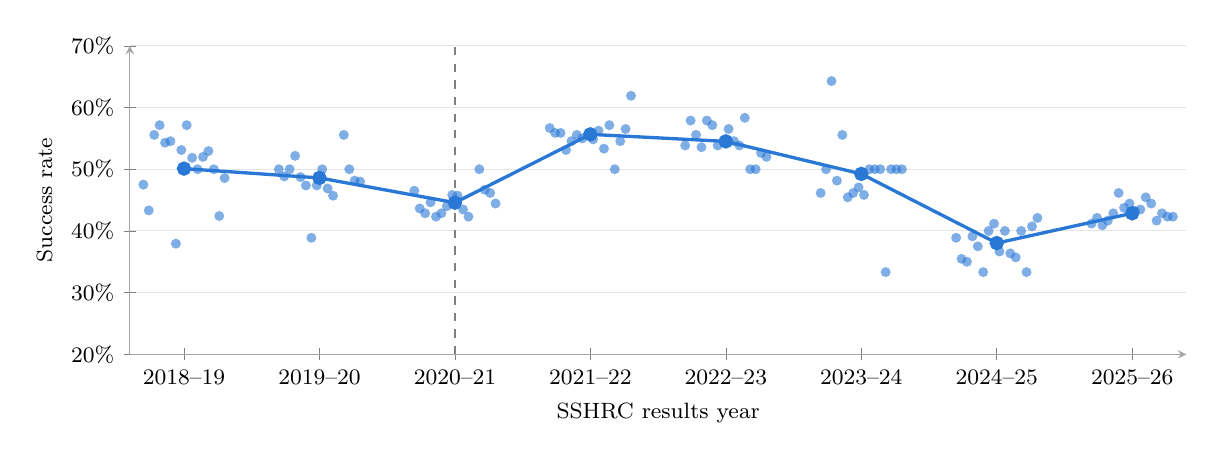
\begin{tikzpicture}
\begin{axis}[
  width=15cm, height=5.5cm,
  xmin=2017.6, xmax=2025.4, ymin=20, ymax=70,
  xtick={2018,2019,2020,2021,2022,2023,2024,2025}, xticklabels={2018--19,2019--20,2020--21,2021--22,2022--23,2023--24,2024--25,2025--26},
  axis x line=bottom, axis y line=left, axis line style={gray!70},
  ymajorgrids, grid style={gray!20},
  tick label style={font=\footnotesize}, label style={font=\footnotesize},
  xlabel={SSHRC results year}, ylabel={Success rate}, ylabel style={align=center},
  clip=false,
  ytick distance=10, yticklabel={\pgfmathprintnumber{\tick}\%},
]
\draw[gray, dashed, line width=0.7pt] (axis cs:2020,20) -- (axis cs:2020,70);
\addplot[only marks, mark=*, mark size=1.8pt, color=sshrcA,
  mark options={fill opacity=0.6, draw opacity=0}]
  coordinates {(2018.18,52.94) (2018.26,42.42) (2018.06,51.85) (2018.10,50.00) (2018.14,52.00) (2017.78,55.56) (2017.90,54.55) (2017.74,43.33) (2018.30,48.57) (2018.22,50.00) (2017.82,57.14) (2017.70,47.50) (2018.02,57.14) (2017.94,37.93) (2017.98,53.12) (2017.86,54.29) (2019.18,55.56) (2019.26,48.15) (2019.06,46.88) (2019.10,45.71) (2018.78,50.00) (2018.90,47.37) (2018.74,48.84) (2019.30,48.00) (2019.22,50.00) (2018.82,52.17) (2018.70,50.00) (2019.02,50.00) (2018.94,38.89) (2018.98,47.37) (2018.86,48.72) (2019.70,46.51) (2019.74,43.64) (2019.78,42.86) (2019.82,44.64) (2019.86,42.31) (2019.90,42.86) (2019.94,44.00) (2019.98,45.83) (2020.02,45.71) (2020.06,43.48) (2020.10,42.31) (2020.18,50.00) (2020.22,46.67) (2020.26,46.15) (2020.30,44.44) (2020.70,56.67) (2020.74,55.88) (2020.78,55.88) (2020.82,53.12) (2020.86,54.55) (2020.90,55.56) (2020.94,55.00) (2020.98,55.56) (2021.02,54.84) (2021.06,56.25) (2021.10,53.33) (2021.14,57.14) (2021.18,50.00) (2021.22,54.55) (2021.26,56.52) (2021.30,61.90) (2021.70,53.85) (2021.74,57.89) (2021.78,55.56) (2021.82,53.57) (2021.86,57.89) (2021.90,57.14) (2021.94,53.85) (2021.98,54.55) (2022.02,56.52) (2022.06,54.55) (2022.10,53.85) (2022.14,58.33) (2022.18,50.00) (2022.22,50.00) (2022.26,52.63) (2022.30,52.00) (2022.70,46.15) (2022.74,50.00) (2022.78,64.29) (2022.82,48.15) (2022.86,55.56) (2022.90,45.45) (2022.94,46.15) (2022.98,47.06) (2023.02,45.83) (2023.06,50.00) (2023.10,50.00) (2023.14,50.00) (2023.18,33.33) (2023.22,50.00) (2023.26,50.00) (2023.30,50.00) (2023.70,38.89) (2023.74,35.48) (2023.78,35.00) (2023.82,39.13) (2023.86,37.50) (2023.90,33.33) (2023.94,40.00) (2023.98,41.18) (2024.02,36.67) (2024.06,40.00) (2024.10,36.36) (2024.14,35.71) (2024.18,40.00) (2024.22,33.33) (2024.26,40.74) (2024.30,42.11) (2024.70,41.18) (2024.74,42.11) (2024.78,40.91) (2024.82,41.67) (2024.86,42.86) (2024.90,46.15) (2024.94,43.75) (2024.98,44.44) (2025.02,43.24) (2025.06,43.48) (2025.10,45.45) (2025.14,44.44) (2025.18,41.67) (2025.22,42.86) (2025.26,42.31) (2025.30,42.31)};
\addplot[color=sshrcA, line width=1.2pt, mark=*, mark size=2pt] coordinates {(2018.00,50.10) (2019.00,48.59) (2020.00,44.58) (2021.00,55.65) (2022.00,54.51) (2023.00,49.24) (2024.00,38.03) (2025.00,42.86)};
\end{axis}
\end{tikzpicture}
